%!TEX root = ../01-Quantum-Hall-Effect.tex
\chapter{Theoretical Preliminaries}\label{chap:theory}

\section{Two Dimensional Electron Gas (2DEG)} \label{sec:2deg-theory}
\begin{figure}
	\centering
	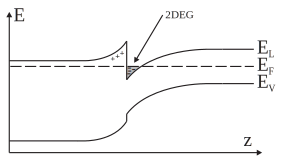
\includegraphics[width=.5\textwidth]{./img/bandstructure-GaAs.pdf}
	\caption[Band structure of AlGaAs-GaAs heterostructure]{\textbf{Band structure of AlGaAs-GaAs heterostructure} The different chemical potentials create a bend in the band edges of the heterostructure, forming a thin, triangular quantum well below the Fermi level\par Source: \url{https://www.nano.physik.uni-muenchen.de/nanophotonics/_assets/pdf/f1/K1_QHE_Anleitung_deutsch.pdf}}
	\label{fig:bandstructure_GaAs}
\end{figure}
In a two dimensional electron gas, the movement of electrons is confined to a plane, thus leading to quantized levels of motion in the third direction.
For the most problems, these levels can then be ignored.
One way of creating such a 2DEG is the employment of semiconductor-oxide-interfaces.
\autoref{fig:bandstructure_GaAs} shows the band structure of such an AlGaAs-GaAs-junction.
Since the band edges of the materials differ vastly, a thin triangular potential well is formed with its minimum below the Fermi level, effectively confining the electrons to a small region around the junction.
Hence, for low enough temperatures, only the lowest level of the quantum well is occupied and so the motion perpendicular to the junction surface can safely be ignored.
However, the electron still is free to move in a direction parallel to the junction, effectively realizing a 2DEG.

The dispersion relation of a 2DEG is
\begin{equation}\label{eq:subband}
	E_{k_\text{x}, k_\text{y}} = E_\text{s} + \frac{\hbar^2}{2m_\text{eff}}\left(k_\text{x}^2 + k_\text{y}^2\right),
\end{equation}
where $E_\text{s}$ is the ground state energy of the quantum well.

The density of states is calculated by counting the states in k-space
\begin{equation*}
	N(\epsilon) = \underbrace{2}_{\text{spin degeneracy}}\cdot\frac{\pi k^2\cdot S}{4\pi^2} = S\frac{2m_\text{eff}\cdot\epsilon}{2\pi\hbar^2} = S\frac{m_\text{eff}\cdot\epsilon}{\pi\hbar^2}.
\end{equation*}
and differentiating with respect to energy
\begin{equation}\label{eq:dos}
	\nu(\epsilon) = \frac{1}{S}\cdot\diff[N(\epsilon)]{\epsilon}\theta(\epsilon-E_0) = \frac{m_\text{eff}}{\pi\hbar^2} = \text{const.}.
\end{equation}

\section{2DEG In a Magnetic Field}\label{sec:mag_2deg}
We want to solve the stationary Schrödinger Equation
\begin{equation*}
	\frac{1}{2m_\text{eff}}\left(\vec{p}-e\vec{A}\right)^2\psi = E\psi.
\end{equation*}
In Lorentz gauge, we can choose $\vec{A}=(0, Bx, 0)^T$ and solve by a product ansatz $\psi(x,y,z) = \phi(x,y)Z(z)$.
The z-equation is readily solved with the eigenenergies being the sub-band energies mentioned in \autoref{eq:subband}.
Solving the eigenequation for $\phi(x,y)$ yields the \textit{Landau levels}
\begin{equation*}
	\epsilon_n = \hbar\omega_\text{c}\left(n+\frac{1}{2}\right)\qquad{n\in\mathbb{N}_0},
\end{equation*}
where $\omega_\text{c} = \frac{eB}{m}$ is called the cyclotron frequency.

Additionally, as a result of the electron spin, there is a twofold Zeeman splitting
\begin{equation*}
	E = \epsilon_n + \underbrace{\frac{1}{2}}_\text{electron spin}\cdot g_\text{eff}\mu_\text{B}\cdot B,
\end{equation*}
where $g_\text{eff}$ is the effective Landé factor and $\mu_\text{B}$ the Bohr magneton.

Using \autoref{eq:dos}, the number of electrons occupying a Landau level per unit area is
\begin{equation*}
	N = \hbar\omega_\text{c}\nu(\epsilon) = \frac{2eB}{h}.
\end{equation*}
Calculating the clasically expected Hall voltage $U_\text{H}$, it follows
\begin{align*}
	U_\text{H} = \frac{B}{n_\text{s}\cdot e}\cdot I.
\end{align*}
Now, if all $n=1,\dots,\lambda$ energy levels are fully occupied (thus $n_\text{s}=\lambda N$), the Hall resistance reads
\begin{equation*}
	R_\text{H} = \frac{B}{\lambda N\cdot e} = \frac{h}{\lambda\cdot e^2}\qquad \lambda\in\mathbb{N}.
\end{equation*}
However, the instruments used in this experiment do not allow for a high enough resolution to observe the Zeeman splitting.
Hence, only even-numbered levels can be seen.

\section{Practical Realization of the 2DEG}\label{sec:2deg-irl}
Two samples are provided, which utilize different techniques to confine electrons in a plane.
The first sample is a silicon n-channel MOSFET (metal oxide semiconductor field effect transistor).
The structure, shown in \autoref{fig:2deg-irl:mosfet}, is built on the surface of a p-type doped silicon substrate, with two n-type wells forming the electrical contacts for source and drain.
The source contact is also connected electrically to the substrate.
The region between source and drain is covered with an insulating oxide layer  onto which a metal electrode, referred to as the gate, is deposited.
A voltage applied betweent the gate and source (and therefore the p-type substrate) can attract or repel charge carriers.
If this voltage is positive at the gate and high enough to push the energy level of the conductance band below the fermi energy, a two-dimensional inversion region with an approximate width of \SI{25}{\angstrom} forms in the substrate at the boundary to the oxide layer.
Above this threshold voltage, the gate-source voltage can be used to modulate the charge carrier density inside this inversion layer.
A drawback of this method is that it is yet not possible to create a perfectly planar boundary surface, allowing electrons to scatter on surface irregularities.
Also being located within the doped substrate, the electrons in the 2DEG can scatter on the defects introduced by the doping, further lowering their mobility to approximately \SI{4}{\meter\squared\per\volt\per\second} at \SI{1}{\kelvin}.

Another method, already mentioned in \autoref{sec:2deg-theory}, is the use of a heterostructure of two materials with highly dissimilar band gaps, such as GaAs and AlGaAs.
The provided sample uses pure GaAs and n-type AlGaAs.
The pure GaAs has a narrower band gap than the AlGaAs, leading to the deformation of conductance and valence bands shown in \autoref{fig:bandstructure_GaAs}.
Electrons from the n-type AlGaAs can migrate into the potential well where they are physically separated from the donor atoms.
Also this structure can be produced very precisely using molecular epitaxy, nearly eliminating electron scattering at the surface, leading to a mobility which can be greater than \SI{100}{\meter\squared\per\volt\per\second}.
Another advantage is the slightly lower effective mass inside the GaAs of $m^* \approx \num{0.07} m_\text{e}$ compared to $m^* \approx \num{0.2} m_\text{e}$ in silicon.
In addition to the two contacts used to inject the external current, there are six contacts distributed on either side of the main channel.
These contacts are used to measure the hall voltage and longitudinal voltage without interference from the strongly deformed current flow at high magnetic fields.

\autoref{fig:2deg-irl:hetero}
\begin{figure}
	\centering
	\begin{subfigure}{.4\textwidth}
		\centering
		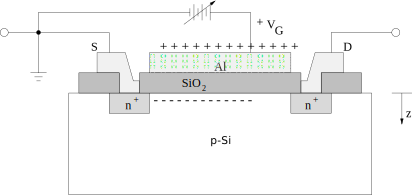
\includegraphics[width=\textwidth]{./img/nfet.pdf}
		\caption{N-channel MOSFET}\label{fig:2deg-irl:mosfet}
	\end{subfigure}
	\begin{subfigure}{.4\textwidth}
		\centering
		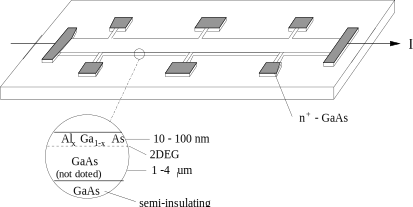
\includegraphics[width=\textwidth]{./img/gaas-heterostructure.pdf}
		\caption{AlGaAs-GaAs heterostructure}\label{fig:2deg-irl:hetero}
	\end{subfigure}
	\caption{\textbf{Schematic illustration of the provided samples}\\Source: experiment instruction}
\end{figure}

\section{Shubnikov-De Haas Effect}
\begin{figure}
	\centering
	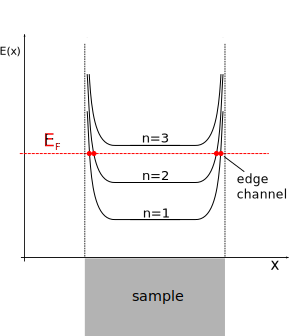
\includegraphics[width=.5\textwidth]{./img/on-edge.pdf}
	\caption[Edge channels of the 2DEG]{\textbf{Edge channels of the 2DEG} As described in \autoref{sec:mag_2deg}, the energy levels are described by Landau levels, bending upwards at the edges of the sample.\par Source: Wikipedia, Shubnikov-de Hass effect}
	\label{fig:on_edge}
\end{figure}

The SdH effect describes an oscillation in the conductivity of a material in the presence of a strong magnetic field at low temperatures.

\autoref{fig:on_edge} depicts the situation, where the Fermi level $E_\text{F}$ is located in between two Landau levels.
Since electrons now only scatter at the edges of the sample, where the Fermi level and the work function intersect, the corresponding states are called \textit{edge channels}.
However, since the conductivity is quantized and a voltage measurement should ideally involve no flowing current, it follows
\begin{equation*}
	I = \frac{\lambda\cdot 2e}{h}(\mu_\text{R} - \mu_\text{L}) \stackrel{!}{=} 0.
\end{equation*}
Therefore, the chemical potentials at the edges must be the same, leading to a vanishing resistance in the edge states.

Letting a Landau level correspond to an edge channel of the sample, at a constant electron density it follows
\begin{equation*}
	B_\lambda = \frac{nh}{2e\lambda}\Rightarrow \Delta\left(\frac{1}{B}\right) = \frac{2e}{nh},
\end{equation*}
yielding the periodic behavior in $\frac{1}{B}$.

\section{Experimental Setup}
The experiment is performed inside a two-stage cryostat.
The first stage is thermally insulated from the environment by a dewar flask and multi-layer insulation.
It contains the inner dewar, which is surrounded by a superconducting coil.
During the experiment it is first filled with liquid nitrogen, then purged and filled back with liquid helium.
The second dewar flask forms the probe chamber, a carbon resistor is used to measure the temperature of the inner chamber.
Both chambers are sealed to allow control of the internal pressures and allow recovery of the evaporated helium.
A capillary hole in the inner flask allows liquid helium to transfer to the inner probe chamber.
To further cool the probe chamber below the boiling point of helium at ambient pressure, a vacuum pump can be used to lower the pressure inside the probe chamber.

The variable magnetic field is provided by the aforementioned superconducting coil.
To quickly switch between the normal and persistent operating modes, a superconducting switch is used.
Heating the switch with a resistive heater brings it above its critical temperature, breaking the loop and allowing the current to be adjusted.

An adjustable constant current supply is used to create a current flow through the probes.
The voltage across various test points, spanning the probe longitudinally and transversely, freely selected with two rotary switches, is measured with a multimeter.
An x-y plotter simultaneously records the relationship between the voltage and magnetic field.
